\documentclass[acmtog, review, anonymous]{acmart}
\acmSubmissionID{558}

\usepackage{booktabs}
\usepackage{natbib}
\usepackage{xspace}
\usepackage[nolist]{acronym}
\usepackage{bm}

%\usepackage{t1enc}
\usepackage{soul}
\usepackage{amsmath}
\usepackage{amssymb}
\usepackage{microtype}
\usepackage{wrapfig}

\def\figurePath{figures/}

\def\myfigure#1#2{\begin{figure}[htb]\centering\includegraphics*[width = \linewidth]{\figurePath#1}\caption{#2}\label{fig:#1}\end{figure}}

\def\mycfigure#1#2{\begin{figure*}[t]\centering\includegraphics*[clip, width = \linewidth]{\figurePath#1}\caption{#2}\label{fig:#1}\end{figure*}}

\newcommand{\mywrapfigure}[3]{%
\begin{wrapfigure}{r}{#2\columnwidth}%
  \begin{center}%
    \includegraphics[width=#2\columnwidth]{\figurePath#1}%
    \vspace{0.0cm}%
    \caption{#3}%
    \label{fig:#1}%
  \end{center}%
\end{wrapfigure}%
\leavevmode%
}

\newcommand{\TR}[1]{\textcolor{blue}{\textbf{TR: #1}}}
\newcommand{\eg}{e.g., }
\newcommand{\ie}{i.e., }

\newcommand{\argmax}[1]{\underset{#1}{\operatorname{arg\,max}}}
\newcommand{\argmin}[1]{\underset{#1}{\operatorname{arg\,min}\ }}
\newcommand{\diag}[1]{\operatorname{diag}(#1)}
\newcommand{\refSec}[1]{Sec.~\ref{sec:#1}}
\newcommand{\refFig}[1]{Fig.~\ref{fig:#1}}
\newcommand{\refEq}[1]{Eq.~\ref{eq:#1}}
\newcommand{\refTbl}[1]{Tbl.~\ref{tbl:#1}}
\newcommand{\refFigStart}[1]{Figure~\ref{fig:#1}}

\newcommand{\unsure}[1]{{\sethlcolor{yellow}\hl{#1}}}

\soulregister\ref7
\soulregister\cite7
\soulregister\refFig7
\soulregister\refFigStart7
\soulregister\cite7
\soulregister\ref7
\soulregister\pageref7
\soulregister\shortcite7
\soulregister\namecite7
\soulregister\eg7
\soulregister\ie7
\soulregister\etal7
\soulregister\reftbl7
\soulregister\name7
\soulregister\unsure7

\DeclareGraphicsExtensions{.png,.jpg,.pdf,.ai,.psd}
\DeclareGraphicsRule{.ai}{pdf}{.ai}{}
\DeclareGraphicsRule{.psd}{pdf}{.psd}{}

\newcommand{\mysection}[2]{\section{#1}\label{sec:#2}}
\newcommand{\mysubsection}[2]{\subsection{#1}\label{sec:#2}}
\newcommand{\mysubsubsection}[2]{\subsubsection{#1}\label{sec:#2}}


\begin{acronym}
\acro{2AFC}{Two-alternative Forced Choice}
\acro{AdaIN}{Adative Instance Normalization}
\acro{BRDF}{Bi-directional Reflectance Distribution Function}
\acro{CNN}{Convolutional Neural Network}
\acro{svBRDF}{Spatially-varying Bi-directional Reflectance Distribution Function}
\acro{VAE}{Variational Auto-encoder}
\end{acronym}

\newcommand{\mymath}[2]{\newcommand{#1}{\TextOrMath{$#2$\xspace}{#2}}}

\mymath{\location}{\mathbf x}
\mymath{\scale}{s}
\mymath{\flashImage}{L}
\mymath{\outgoingDirection}{\omega_\mathrm o}
\mymath{\render}{\mathbf R}
\mymath{\materialModel}{f}
\mymath{\materialModelParameters}{\theta}
\mymath{\lossOld}{\mathcal L'}
\mymath{\textureComparisonOld}{\mathcal T'}
\mymath{\patchOld}{\mathcal P'}
\mymath{\loss}{\mathcal L}
\mymath{\textureComparison}{\mathcal T}
\mymath{\patch}{\mathcal P}
\mymath{\stationarity}{\mathcal S}
\mymath{\materialCode}{\mathbf z}
\mymath{\flashImageEncoder}{g}
\mymath{\expectation}{\mathbb E}
\mymath{\latentDimension}{n_\mathrm z}
\mymath{\spectralWeight}{\lambda}
\mymath{\Zdimension}{128}

\setcopyright{none}

\citestyle{acmauthoryear}
\setcitestyle{square}

\settopmatter{authorsperrow=4}

\begin{document}

\title{Generative Modelling of BRDF Textures from Flash Images}

% Authors.
\author{Philipp Henzler}
\affiliation{%
  \department{Department of Computer Science}
  \institution{University College London}}
\email{p.henzler@cs.ucl.ac.uk}

\author{Valentin Deschaintre}
\affiliation{%
  \institution{Imperial College London}}
\email{v.deschaintre@imperial.ac.uk}

\author{Niloy J. Mitra}
\affiliation{%
  \institution{University College London}}
\email{n.mitra@ucl.ac.uk}

\author{Tobias Ritschel}
\affiliation{%
  \department{Department of Computer Science}
  \institution{University College London}}
\email{t.ritschel@ucl.ac.uk}

\renewcommand{\shortauthors}{Henzler et al.}

% abstract
\begin{abstract}
We learn a space of stationary materials for easy capture, intuitive editing, consistent interpolation, and efficient reproduction of visual material appearance.
To use our system, users provide a photo of stationary natural material captured under flash light illumination, which, in milliseconds, is converted into a latent material code.
These codes can then be manipulated, \eg meaningfully interpolated, semantically edited or compactly stored. 
In a second step, conditioned on the material code, our method produces an infinite and diverse spatial field of BRDF model parameters (diffuse albedo, specular albedo, roughness, normals) that allows rendering in complex scenes and illuminations, matching the appearance of the input picture.
Technically, we jointly embed all flash images into a latent space using a convolutional encoder, and -- conditioned on these latent codes -- convert random spatial fields into fields of BRDF parameters using convolutional neural network (CNN). We condition these BRDF parameters to match the visual characteristics (statistics and spectra of visual features) of the input under matching light.
\end{abstract}

\begin{teaserfigure}
  \centering
  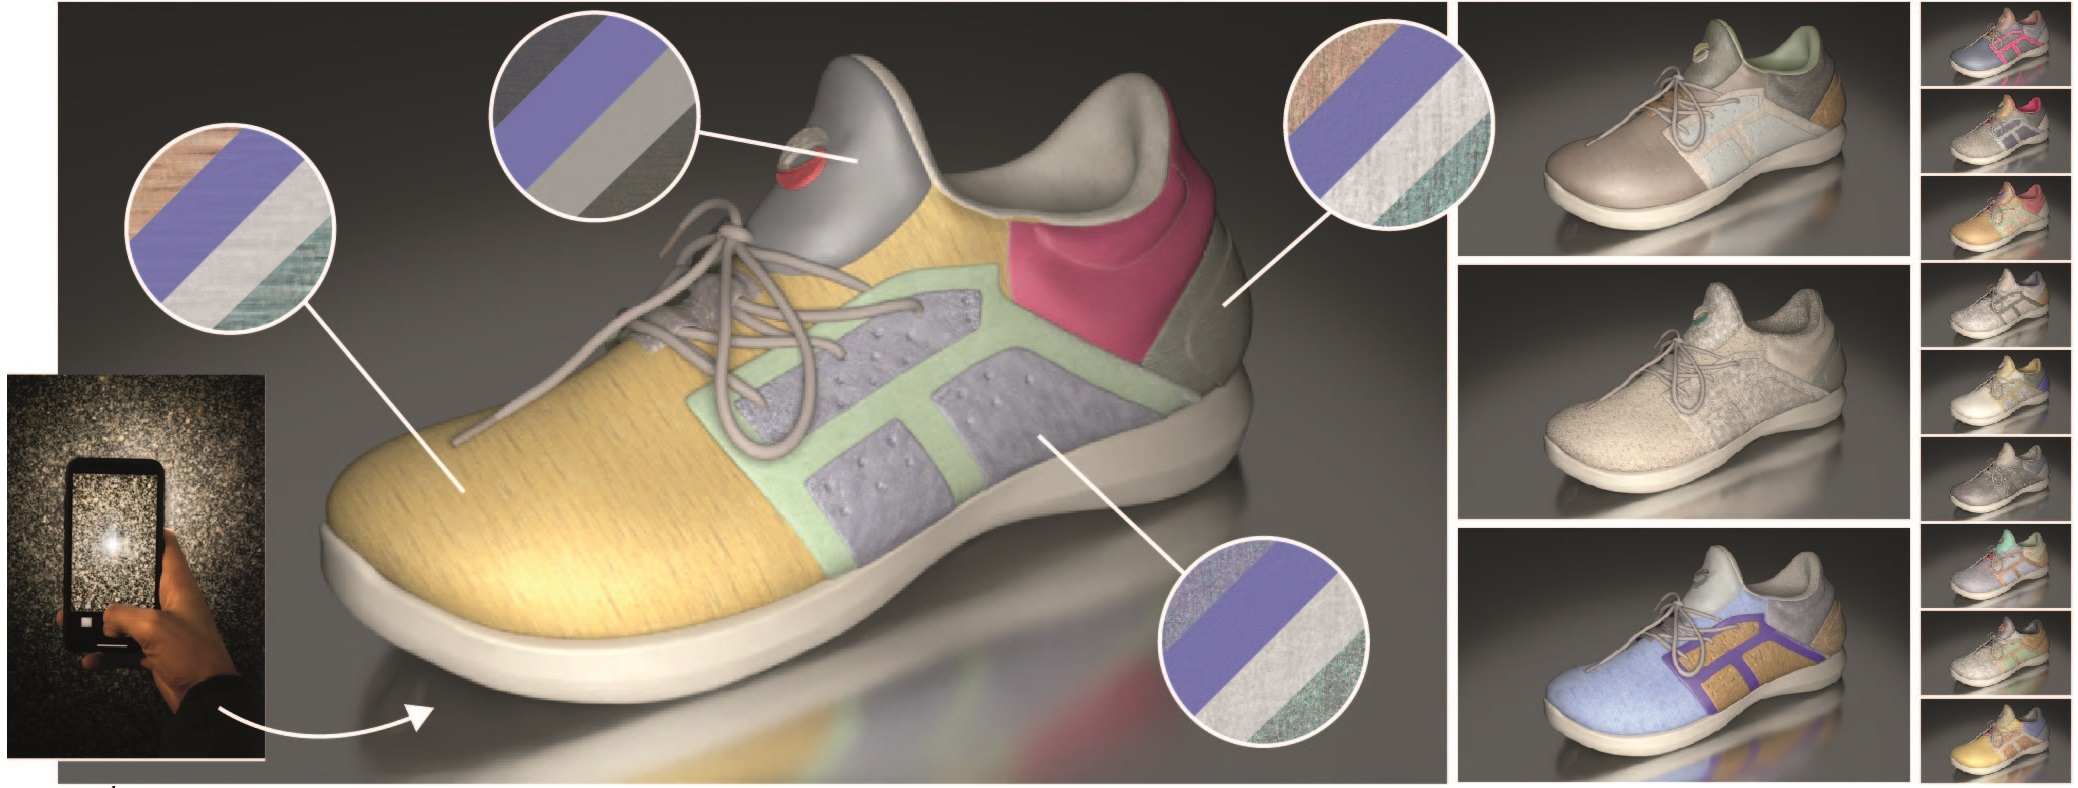
\includegraphics[width=\linewidth]{figures/teaser_current.jpg}
  \caption{Random samples from our generative model of BRDF maps, assigned to a 3D object of a shoe.}
  \label{fig:Teaser}
\end{teaserfigure}

\maketitle

\section{Introduction}
Rendering realistic images for feature films or computer games requires adequate simulation of light transport.
Besides geometry and illumination, an important factor is material appearance.

Material appearance has three aspects of variation:
%
First, when view or light direction change, reflected light changes.
The physics of this process is well-understood and can be simulated provided the right input parameters to a simulation are available.
%
Second, behavior changes across materials.
For example, leather reacts differently to light or view changes than paper would, yet, different forms of leather clearly share visual properties, \ie form a (material) space.
%
Third, appearance details depend on spatial position.
Different locations in the same leather exemplar bahaves differently but all share the same visual statistics \cite{portilla2000parametric}, \ie they form \emph{texture}.

Classic computer graphics captures appearance by \emph{reflection models}, which predict for a given i)~light-view configuration, ii)~material, and iii)~spatial position, how much light is reflected.
%
Typically, the first variation (light and view direction) is covered by \emph{BRDF models}, analytic expressions, such as \citet{phong1975illumination} which map the light and view direction vector to scalar reflectance.
%
The second variation (material) is covered by choosing \emph{BRDF model parameters}, such as Phong glossiness.
In practice, it can be difficult, given a desired appearance, to choose those parameters \eg how to make make a leather look more like fabric.
Measuring BRDF model parameters requires complex capture hardware.
%
The third variation (spatial) is addressed by storing multiple BRDF model parameters in images of finite size --often referred to as \ac{svBRDF} maps-- or writing functional expressions to reproduce their behaviour.
It is even more challenging to choose these parameters to produce something coherent like leather, in particular over a large or even infinite spatial extent.
Additionally, storing all these values requires substantial memory and programming functional expressions to mimic their statistics requires expert skills and time.
Capturing the spatial variation of BRDF model parameters over space using sensors is even more involved \cite{BTF}.

Addressing those issues, we provide a reflectance model to jointly generalize across all of these three axes.
Instead of using analytic parameters, we parametrize appearance by latent codes from a learned space, allowing for generation, interpolation and semantic editing.
Without involved capture equipment, these codes are produced by presenting the system a simple 2D flash image, which is then embedded into the latent space.
Avoiding to store any finite image texture, we learn a second mapping to produce reflectance from the infinite random field (noise) on-the-fly, conditioned on the latent material code. 
Instead of using any advanced capture device for learning, flash images will be the only supervision we use.
%
\myfigure{Space}{From a flash image, which contains sparse observations across material, space and view-light \textbf{(left)}
we map to a latent code \textbf{(middle)}
so that changes in that code can be decoded to enable \textbf{(right)} material synthesis (holding material fixed and moving spatially), material morphing (holding space and view/light fixed and changing material), or classical shading and material generation (points in the latent space).}

A use case of our approach is shown in \refFig{Teaser}.
First, a user provides a ``flash image'' a photo of a flat material sample under flash illumination.
This sample is embedded as a code into a latent space using a CNN.
This code is a very compact description that can be manipulated, \eg interpolated with a different material, changed along semantic axis. 
Previous work has considered spaces of BRDFs \cite{matusik2003data} or RGB textures \cite{matusik2005texture} but no spatial variation of reflectance.
Conditioned on this code, a second CNN can generate an infinite field of BRDF to be directly used in rendering. 

For training, we solely rely on real flash images.
The key insight, inspired by \citet{aittala2016reflectance} is that these flash images reveal the same texture at different image locations -- they are stationary -- but under different view and light angles.
Using this constraint, \citet{aittala2016reflectance} were able to decompose a single input image to capture the parameters of a material model that could then be rendered under novel view or light directions.
However, this covers only part of the generalization we are targeting: it generalizes across view and light, but not across location or material. 
Further, their process requires performing an optimization for every exemplar, requiring order of hours, while our embedding and generation require milliseconds only.

In summary, our main contributions are
\begin{itemize}
\item a generative model of a BRDF material texture space;
\item generation of maps that are diverse over the infinite plane;
\item a flash image dataset of stationary materials enabling our training with no BRDF parameter supervision or synthetic data; and
\item feed-forward embedding of exemplar flash images into the space in milliseconds using a CNN, without per-material optimization. 
\end{itemize}

\mysection{Previous Work}{PreviousWork}
Our work has background in texture analysis, appearance modelling and design spaces. 

\subsection{Textures in Graphics}
A classic definition of texture is defined by \citet{julesz1965texture}: \textit{a texture is an image full of features that in some representation have the same statistics.}
\citet{portilla2000parametric} have provided a practical method to compute representations in to do statistics on.
They use liner filters on multiple scales

\citet{perlin1985noise} was first to capture the fractal \cite{mandelbrot1983fractal} stochastic variation of appearance in model applicable to Computer Graphics.
His approach is simple --a linear combination of noise at different scales-- yet extremely powerful, and has led to extensive use in computer games or production rendering.
Wavelet noise \cite{cook2005wavelet} moved this idea further by band-limiting the noise that is combined.
Such methods can be used of materials, \eg for gloss maps, bump maps, etc.
Regrettably, it does not provide a solution to acquire a texture from an exemplar, which is left to manual adjustment.

To generate textures from exemplars, non-parametric sampling \cite{efros1999texture}, vector quantization \cite{wei2000fast}, optimization \cite{kwatra2005texture} or nearest-neighbour field synthesis (PatchMatch \cite{barnes2009patchmatch}) have been proposed.
These work well in images, but are used less in production rendering or games, due to issues in computational scalability and lack of intuitive control.

The word ``texture'' can be ambiguous to mean stochastic variation, as well as images attached on surfaces to localize color features.
The voxels used by \citet{zhu2018visual} and MLPs used by  \citet{oechsle2019texturefields} represent diffuse albedo, and refer to the localized color appearance, \eg wheels of a car are dark, the rim are silver, etc., as ``texture''.
Here, we focus on stochastic variation in the sense of \citet{julesz1965texture} or \citet{portilla2000parametric}.

Our approach will build on deep learning-based texture synthesis 
\cite{simonyan2014very,gatys2015texture,sendik2017deep,ulyanov2016texture,johnson2016perceptual,ulyanov2017improved,shaham2019singan,bergmann2017learning,zhou2018non,karras2019style}.
Besides applying them to BRDFs, we extend these ideas.
We detail their background in \refSec{TextureSynthesis}

\subsection{Material Modeling}
Representing appearance in simulation-based graphics has been an activate research field for decades.
The survey by \citet{guarnera2016brdf} present detailed discussion of the many different material model and BRDF acquisition approach.
In our method, we use a state-of-the-art micro-facet BRDF model \cite{cook1982reflectance}, and focus here on deep-learning based material modelling and acquisition.

Many methods have been proposed to acquire materials using data driven approaches.
\citet{matusik2003data} proposed a data driven BRDF model, using a linear model. More recently, \citet{rematas2016deep} extract reflectance maps from 2D images using a CNN trained is a supervised manner. Materials and illuminations acquisition were further explored by \citet{georgoulis2017reflectance}.
\citet{deschaintre2018single} proposed a rendering loss to capture svRBDFs from flash images.
Pix2Pix \cite{pix2pix2016} inspired many other approaches for image to image translation to translate RGB pixels to material attributes \cite{li2018learning,li2017modeling,li2018materials}.
Most work however now include a differentiable shading step \cite{liu2017material,li2018learning,deschaintre2018single, deschaintre2019flexible,guo2020materialgan} such as we do here.
\citet{gao2019deep} proposed to use a post-optimization in an encoded latent space, improving an initial material estimation, and comparing renderings of their results directly to their input pictures.
All these approaches focus on capturing a single instance of a \ac{svBRDF} map, but with little or no editing options across materials (space) or generalization across the spatial domain (diversity).
\citet{kuznetsov2019learning} modeled an important aspect of physically-based rendering using adversarial training: the Normal Distribution Function (NDF).

We take inspiration from \citet{aittala2016reflectance} who extended the approach of \citet{gatys2015texture} to generate \ac{svBRDF} parameter maps from a single picture of a stationary material exemplar.

\subsection{Spaces-of}
Spaces of color \cite{nguyen2015data}, materials \cite{matusik2003data}, textures \cite{matusik2005texture}, faces \cite{blanz1999morphable}, human bodies \cite{allen2003space}, and more have been useful in graphics.
% 
Closest to our approach, \citet{matusik2005texture} has devised a space of textures.
Here, users can interpolate combinations of visually similar textures.
They warp all pairs of exemplars to each other and constructs graph edges for interpolation when there is evidence that the warping is admissible.
To blend between them, histogram adjustments are made.
Consequently, interpolation between exemplars does not take a straight path in pixel space from one to the other, but traverses only valid regions.
Photoshape \cite{park2019photoshape} learns the relation of given material textures over a database of 3D objects.

\mysection{Background}{Background}

\mysubsection{Flash Images}{Flash Images}
\citet{aittala2016reflectance} leveraged the fact that a single flash image of a stationary material reveals multiple realizations of the same reflectance statistics under different light and view angles.
We will now recall a simplified definition of their approach. 

A flash image is an RGB image of a material, taken in conditions where the phone's flashlight is the dominant light source.
We write $\flashImage(\location)$ to denote the RGB radiance value at every image location \location.
The image is assumed to be taken in ---or converted to--- linear space.
The illumination is assumed to be an isotropic point light collocated with the camera.
Further, the geometry is assumed to be flat and captured in a fronto-parallel setting, so that the direction from light to every image location in 3D is known.
Self-occlusion and parallax are assumed to be negligible.\\
Reflectance is parametrized by a \emph{material}, represented as a function $\materialModel(\location)$ mapping image location \location to shading model parameters --including the shading normal.
Under these conditions, the reflected radiance is
$
\flashImage=\render\materialModel
$, where \render is the \emph{differentiable} rendering operator, mapping shading model parameters to radiance.

A material \materialModel explains a flash image \flashImage if it is \emph{visually similar} to \flashImage when rendered.
Unfortunately, without further constraints, there are many materials to explain the flash image.
This ambiguity can be resolved when assuming that the material \materialModel is \emph{stationary}.
We say a material is stationary, if local statistics of the shading model parameters $f$ do not change across the image.
  
Putting both --visual similarity and stationarity-- together, the best material from a family $\materialModel_\materialModelParameters$ of material mapping functions parametrized by a vector \materialModelParameters, can be found by minimizing a loss:
\begin{align}
\label{eq:ImageLoss}
\lossOld(\materialModelParameters):=
\textureComparison(
\flashImage,
\render\materialModel_\materialModelParameters)
+
\lambda
\stationarity(\materialModel_\materialModelParameters)
,
\end{align}
where $\textureComparison(\flashImage,\render\materialModel_\materialModelParameters)$ is a metric of visual similarity between a flash image $\flashImage$ and a differentiable rendering $\render\materialModel_\materialModelParameters$, and $\stationarity(\materialModel)$ is a measure of stationarity of a material map \materialModel.

Comparison, \textureComparison, of two textures is not trivial.
Pixel-by-pixel comparison is typically not suitable to evaluate visual statistical similarity.
Instead, images are mapped to a feature space in which images that are perceived as similar textures, map to similar points~\cite{portilla2000parametric}.
Different mappings are possible here.
Classic texture synthesis \cite{heeger1995pyramid} uses moments of linear multi-scale filters responses.
\citet{gatys2015texture} proposed to use Gram matrices of non-linear multi-scale filters responses such as those of the VGG \cite{simonyan2014very} detection network.
Such a characterization of textures was also used by \citet{aittala2016reflectance} and, without loss of generality, will be used and extended in this work as well.\\
While \materialModel is stationary, \flashImage is not and has features at different random positions \location which are compared as
\begin{equation}
\textureComparisonOld(\flashImage_1,\flashImage_2)
:=
\expectation_{\location\sim(0,1)^2,\scale\sim(0,1)}[
|
\patch(\flashImage_1,\location)
-
\patch(\flashImage_2,\location)
|_1 ],
\end{equation}
where $\patchOld(\flashImage, \location)$ crops a patch at the location \location resamples it to the input resolution of VGG \cite{simonyan2014very}, computes the filter responses and ultimately their Gram matrices:
\begin{equation}
\patch(\flashImage,\location):=
\mathtt{gram}(\mathtt{vgg}(\mathtt{resample}(\mathtt{crop}(\flashImage,\location, s)))).
\end{equation}
Here, \scale is a scale parameter chosen by the user reprwsenting the size of the crop.

Minimizing \materialModelParameters with respect to \refEq{ImageLoss} for a given \flashImage results in a set of material maps.
$\materialModel_\materialModelParameters$ can represent different approaches.
\citet{aittala2016reflectance} directly use the pixel based optimization, and optimize discrete material maps for \materialModelParameters using a single input flash image \flashImage.
With their approach, optimizing for both visual similarity and stationarity is challenging.
In particular, the reflectance stationarity term \stationarity, requires a ``spectral preconditioning'' step.
Instead, we propose a novel approach in the form of a \unsure{neural} model \materialModel that is (i) valid on an infinite domain and (ii) is stationary by construction.
Thus, our loss does not include the stationarity term.

Next, we describe how to generate RGB textures using deep learning (\refSec{TextureSynthesis}), before combining the two components (flash images and NN texture (spaces)) into our approach (\refSec{OurApproach}).



\mysubsection
{Deep Texture Synthesis}
{TextureSynthesis}
\citet{julesz1965texture} define textures by their feature statistics across space. The choice of which features to use remains an important open problem.
%more specifically activations of filters learned in deep convolutional neural networks \cite{simonyan2014very} (VGG),
With the advent of deep learning, \citet{gatys2015texture} suggested to use Gram matrices of these activations of filters, learned in deep convolutional neural networks (\eg VGG~\cite{simonyan2014very}), for neural style transfer. By optimizing directly over pixel values, their method can produce images with the desired texture properties.
\citet{aittala2016reflectance} rely on the same statistics to recover material parameters of stationary materials.
These methods however requires a different optimization to be ran for each different materials.
%-- which takes two hours per exemaplr for \citet{aittala2016reflectance} -- 

Another group of recent methods \cite{ulyanov2016texture, johnson2016perceptual} introduce neural networks capable of producing RGB textures directly, in milliseconds.

While these approach use a network to generate the textures, they are still limited to the input texture exemplar, and do not show further variations in their results.
\citet{ulyanov2017improved} introduced an explicit diversity term enforcing results in a batch to be different.
This diversity is however limited and restrict the results quality. Indeed, they add a diversity term to the loss, but the architecture is not modified to enable it.\\
Alternatively,  adversarial training has been used to capture the essence of textures \cite{shaham2019singan, bergmann2017learning}, including the non-stationary case \cite{zhou2018non} or even within a single image \cite{shaham2019singan}.
In particular, StyleGAN \cite{karras2019style} generates images with details by transforming noise using adversarial training.
As opposed to these approach we do not rely on challenging adversarial trainings, by directly learning a Neural Network to produce VGG statistics.

Instead of incentivizing stationarity in the loss, \citet{henzler2019learning} suggest a learnable texture representation that is built on mapping an infinite noise field to a field that has the statistics of the exemplar texture.
Their method is a point operation, implemented by an MLP that is fed exclusively with noise sampled at different scales as done by \citet{perlin1985noise}.
By explicitly preventing the network to access any absolute position, this approach is stationary by-design.

\mysection{Noise to BRDF Texture Spaces}{OurApproach}

\mycfigure
{Architecture}
{Our architecture.
Starting from an exemplar, \textbf{(left)}, training extracts a crop \textbf{(black)} and compute VGG Statistics on it.
These are compared in $L_2$ to the statistics of our result, computed by shading material parameter maps \textbf{(right)}.
These maps are produce by executing the point operation MLP \textbf{(blue)}, to map the values of scaled transformed random fields to BRDF model parameters.
An encoder conditions this MLP with the latent material code $\mathbf z$.
Back-propagation occurs from the $L2$ loss to both MLP and encoder, \ie they are learned jointly.
The crop of one area in the flash image corresponds to the same random light-view direction that also is used for shading \textbf{(pink)}.
Similarly, randomly sampled materials and noise fields are used in training.
}

An overview of our approach is shown in \refFig{Architecture}.
We train a neural network which acts as a decoder 
$
\materialModel_\materialModelParameters(\location|\materialCode)
$
that generalizes across spatial positions \location as well as across materials, expressed as latent material codes \materialCode.
The material codes \materialCode are produced by an encoder \flashImageEncoder with $\materialCode= \flashImageEncoder(L)$.
Both encoder and decoder are trained jointly over a set of flash images using the loss:
\begin{align}
\label{eq:Loss}
\loss(\materialModelParameters)
:=
\expectation_{\flashImage}
[
\textureComparison(
\flashImage, 
\render\materialModel_\materialModelParameters(\cdot|\flashImageEncoder_\materialModelParameters(\flashImage))
)
].
\end{align}
This equation is an adapted version of \refEq{ImageLoss} to fit our objectives.
In particular we propose a neural network-based $\materialModel_\materialModelParameters$, leveraging the expectation $\expectation_{\flashImage}$ over all flash images in our training set and removing the stationarity term as it is enforced by construction in our network architecture.
We describe the flash image encoder \flashImageEncoder (\refSec{Encoder}), the material texture decoder \materialModel (\refSec{Decoder}) and the texture comparison model \textureComparison (\refSec{TextureComparison}), next.

\mysubsection{Encoder}{Encoder}
The encoder \flashImageEncoder maps a flash image \flashImage to a latent code \materialCode.
It is implemented using a CNN.
The CNN starts at a resolution of \unsure{1024}$\times$\unsure{1024} and maps to a compact latent code using a ResNet18 \cite{he2016deep}.
Empirically, we find a $\latentDimension=$ \Zdimension\unsure{-dimensional} latent space to work best for our data and present all results using this number.

\mysubsection{Decoder}{Decoder}
The decoder \materialModel maps location \location, conditioned on a material code \materialCode to a set of material parameter maps.
The key idea is to provide the architecture with access to noise, as previously done for style transfer \cite{huang2017arbitrary}, generative modelling \cite{karras2019style} or 3D texturing \cite{henzler2019learning}.
In particular, we sample rectangular patches with edge length of $n\times m$ pixels from an infinite random field and convert them to material maps using a \ac{CNN}.
The \ac{CNN} starts at the desired output resolution $n\times m$ and reduces resolution \unsure{four times} before expanding it to $n\times m$ again.
Let $F$ be the array of input features.
For $i=0$, the first level, in full resolution, these features are sampled from the random field at \location.
Then the output features $F'$ are \begin{align}
F':=
\mathtt{adaIN}(\mathtt{conv}_\theta(F), \mathsf T_\theta\materialCode),
\end{align}
where
$\mathtt{adaIN}$ is \ac{AdaIN} \cite{huang2017arbitrary}, 
$\mathtt{conv}$ a convolution (including up- or down-sampling and non-linearity) and $\mathsf T$ is an affine transformation.
Components with learned parameters are denoted with subscript $\theta$.

\ac{AdaIN} is defined by \citet{huang2017arbitrary} as
\begin{align}
\mathtt{adaIN}(\bm\xi, \{\bm\mu, \bm\sigma^2\})=\frac{\bm\sigma}{\bm\sigma_F}(\bm\xi-\bm\mu_F)+\bm\mu
\end{align}
and remaps the input features with mean $\bm\mu_F$ and variance $\bm\sigma_F^2$ to a distribution with mean $\bm\mu$ and variance $\bm\sigma^2$.

The affine mapping $\mathsf T$ is implemented as  $(\latentDimension+1)\times(2\times c_i)$ matrices multiplied with the latent code -- augmented with a 1 in dimension $\latentDimension+1$. Here $2\times c_i$ represent a different mean and variance for each channel dimension $c_i$ of a layer.
It provides the link between the material code and the noise statistics.
Each material code \materialCode is mapped to a mean and variance to control how the statistics of features are shaped at every channel on every layer of the decoder.\\
Our control of noise statistics from latent codes is similar to StyleGAN \cite{karras2019style}, with the key difference that we do not sample noise at different scales, but learn how to produce noise with different, complex, characteristics at different scales by repeatedly filtering it from high resolutions.

\mysubsection{Images Comparison}{TextureComparison}
We propose to compare images based on a loss that accounts both for the statistics of activations \cite{gatys2015texture} and their spectrum \cite{liu2016texture} on multiple scales and across the infinite spatial field, as in
\begin{equation}
\textureComparison(\flashImage_1,\flashImage_2)
:=
\expectation_{\location\sim\mathbb R^2,\scale\sim(s_\mathrm{min},s_\mathrm{max})}[
|
\patch(\flashImage_1,\location,\scale)
-
\patch(\flashImage_2,\location,\scale)
|_1 ].
\end{equation}
with 
\begin{align}
\patch(\flashImage,\location,\scale)&:=
\mathtt{gram}(V) + \spectralWeight\cdot\mathtt{powerSpectrum}(V)\\
V&:=\mathtt{vgg}(\mathtt{resample}(\mathtt{crop}(\flashImage,\location, s)))
\end{align}
\paragraph{Spectrum}
VGG Gram matrices capture the frequency of a feature appearance, unless it forms a regular pattern \cite{liu2016texture}.
\unsure{ABC et al.} proposed to include the L1 norm of the power spectra of two RGB images into the texture metric for learning a single texture.
We therefore combine both ideas and use VGG, but do not limit ourselves to its statistics, and also leverage its spectrum.

\paragraph{Scale}
As VGG works at a specific scale of features it was trained for, it behaves differently at different scales. As the material should be visually plausible regardless of its scale we include \unsure{multiple} scales \scale, ranging from $\scale_\mathrm{min}=0$ to $\scale_\mathrm{max}=1$ in the loss computation.

\paragraph{Infinity}
Expectation over the infinite plane is implemented by simply training with different random seeds for the noise field. This results in the generation of statistically similar, but locally different variations of materials.
As, given a seed, every generated patch is a coherent material, combinations of multiple patches remains coherent as well.
This allows to query an endless, seamless and diverse stream of patches without repetition.

\mysubsection{Material model}{MaterialModel}
We use the Cook-Torrance \shortcite{cook1982reflectance} micro-facet BRDF Model, with Smith's geometric term \cite{heitz2014understanding}, Schlick's \shortcite{schlick1994inexpensive} Fresnel and GGX \cite{walter2007microfacet}.
Hence, parameters are diffuse albedo, specular albedo, roughness and height, \ie eight dimensions. For practical purposes we differentiate height into normal vectors.

\mysubsection{Alignment}{Aligment}
We find that many flash images entail a slight rotation as it can be difficult to take a completely fronto-parallel image.
This was handled by \citet{aittala2016reflectance} by locating the brightest pixel and cropping, but we found our, more abstract, training to struggle with such solution.

Instead, we add a horizontal and a vertical rotation angle to the parameter vector generated from the latent code (not shown in \refFig{Architecture} for clarity).
During training, these are used to rotate the plane, including the normals.
During testing, these angles are not applied meaning that the output is in the local space of the exemplar.

We use a branch of the encoder to perform the alignment task, allowing to jointly align all images based on their visual features \unsure{by committing to some regularized network parameters}.

A byproduct is that the encoder returns angular distance to fronto-parallelity, which could be used to guide users during capture.

\mysubsection{Training}{Training}
For better generalization, we train the syetem as a \ac{VAE} \cite{kingma2013auto}, so instead of mapping to a single \Zdimension-D latent material code, the encoder \flashImageEncoder maps to a \Zdimension-D mean and variance vector, from which we sample in training.
At test time we use the mean for each \Zdimension-D.
We have omitted the additional \ac{VAE} terms enforcing \materialCode to be normally distributed from \refEq{Loss} for clarity.

\mysection{Results}{Results}

\mysubsection{Dataset}{Dataset}
We have created an extended dataset of flash images for testing and training of our approach.
It comprises of \unsure{500} images.
We reserve \unsure{100} images of testing, augmented by all images from \citet{aittala2016reflectance}.
Hence, no image from \citet{aittala2016reflectance} was seen during training.
A subset of the training data was manually labeled with semantic classes to be used in \refSec{}

\mysubsection{Quantitative Evaluation}{Quantitative}
For quantitative analysis we compare our approach to a range of alternative methods in respect to different metrics.

\subsubsection{Comparison}
We compare to three methods by (i)~\citet{aittala2016reflectance}, (ii)~\citet{deschaintre2018single}, and (iii)~\citet{li2018materials}.
We use the BRDF parameter maps provided by \citet{aittala2016reflectance}, executed the code made available by \citet{deschaintre2018single}, and were kindly provided results by \citet{li2018materials} upon request.
We re-render all results using our rendering, making adjustments for gamma and details of representations used by others.
As \citet{li2018materials} require a manual choice of electric and conductor to decide the index of refraction to be used in the Fresnel term, we bound their quality from below by using an oracle: we report the minimal error out of the two interpretations.
Examples are shown in \refFig{Comparison}. 

\subsubsection{Dataset}
Our dataset combines 9 flash images we have captured with the dataset of \citet{aittala2016reflectance} (72 images).

\subsubsection{Metrics}
We quantify style, diversity, and computational speed.
Style is captured by L2 difference of the VGG Gram matrices on patches rendered under random view and light conditions.
A good agreement in style has a low number \ie less is better.
Diversity is captured as the mean pairwise VGG MSE across all realizations.
Here, more is better.
Finally, we measure compute time, where less is better.

\myfigure{ResultsPlot}{Ordered error plot comparing four methods (colors).
Each curve is produced by sorting the errors of each method.
The median can be compared in the middle.
The vertical axis is logarithmic error (less is better).
The horizontal axis is rank (low error left, high error right.)}

\subsubsection{Results}
Results are shown in \refFig{ResultsPlot}.
We see that methods which decompose individual exemplars into shading channels have the lowest error, where \citet{deschaintre2018single} performs better than \citet{li2018materials}.
The approach of \citet{aittala2016reflectance} performs slightly worse than all others, except at the very end of the spectrum, \ie our high errors are higher than theirs.

\begin{table}
\setlength{\tabcolsep}{3pt}
\caption{Comparison of different methods.}
\label{tbl:Results}
\centering
\begin{tabular}{rrrrr}
    \multicolumn{1}{c}{Method}&
    \multicolumn{1}{c}{Error}&
    \multicolumn{1}{c}{Divers.}&
    \multicolumn{1}{c}{Time}&
    \multicolumn{1}{c}{Dim.}
    \\
    \toprule
    \citet{aittala2016reflectance}&5.62&0&h&2D\\
    \citet{li2018materials}&2.26&0&s&2D\\ 
    \citet{deschaintre2018single}&0.62&0&s&2D\\
    Ours&2.92&36.6&ms&2/3D\\
    \bottomrule
\end{tabular}
\end{table}

Note, that only our approach and \citet{aittala2016reflectance} produce a stationary result and that only our result is diverse, \ie we produce infinitely many realizations of a texture while all other approaches produce only one.
Thus, diversity is zero for all other, while it is a constant for ours.
We summarize this in \refTbl{Results}.

In terms of computational speed, \citet{aittala2016reflectance} report two hours of compute time for each per-exemplar optimization to produce a stationary texture, while the image-translation methods are fast, executing only a decoder (less than a second), but do not produce a stationary texture.
Our approach produces one million pixels in milliseconds and without additional memory.

\mycfigure{Comparison}{Comparison of our results to methods that decompose an image into BRDF parameters \textbf{(columns)} for different flash images \textbf{(rows)}.}

\mysubsection{Qualitative Evaluation}{Qualitative}

Example results of our approach are depicted in \refFig{ResultOverview}.
We see that our approach captures a range of different textures, reproducing the style, yet being diverse to produce an infinite field of values.
Interpolation of latent BRDF texture codes is shown in \refFig{Interpolations}.
This figure further shows generalization across space: the input exemplar has a certain size, while the interpolated field of BRDF parameters is much larger, and, with the same latent code or not, could extend forever.
Please see the captions for additional discussion.
\refFig{Teaser} shows examples of generating 3D procedural material textures from 2D inputs.
We see that the model fills space nicely without being bound by a 2D parametrization of the 3D sphere.

The visual quality is best inspected from our interactive WebGL demo in the supplemental.
It allows exploring the space by relighting, changing the random seed and visualizing individual BRDF model channels and their combinations.
The same package contains all channels of all materials as images.
A capture of using the application is further available as an additional supplemental video.

\mycfigure{ResultOverview}{
Result produced by our method for four materials.
For each material we show the flash image left, followed by insets showing crops of the diffuse, specular, roughness and normal channel, followed by a re-rendering.
Please note, that our results share the view-light dependent, yet they do not repeat.
}

\mycfigure{Interpolations}{Interpolation of latent BRDF texture codes.
In each row, a left and a right latent code $\mathbf z_1$ and $\mathbf z_2$ are obtained by encoding two flash images, respectively.
The intermediate, continuous field of BRDF parameters is computed by interpolating from $\mathbf z_1$ to $\mathbf z_2$ and conditioning the decoder MLP with the intermediate code.
The result is lit with five light sources to demonstrate the changes in appearance.
Note how structures emerge and disappear: elements do not simply fade in or out, but their ordinality and shape changes during interpolation.}

\mysection{Semantic Material Control}{SemanticControl}
Our approach allows to embed flash pictures into material codes that can be decoded to corresponding material maps. Furthermore, every random latent material code results in a plausible material.
Yet this is not enough for intuitive manipulation of those codes.
Given a material code \materialCode, we now explore how we can modify it to perform high level semantic control (\eg making a material more leather-like) on the recovered material.

We curate our dataset with the classes \texttt{wood},
\texttt{leather},
\texttt{stone},
\texttt{fabric},
\texttt{cloth},
and
\texttt{plastic}.
For every class we compute the direction $\mathbf n_C$ in latent space that is normal to a plane best separating the in-class and out-class exemplars.
If $C$ is the set of all indices of exemplars in the class, this is \[
\mathbf n=
\expectation_{i\in C}[\materialCode]-
\expectation_{i\not\in C}[\materialCode]
\]
a vector pointing from the barycenter of class $C$ to the barycenter of the non-class.
This allows to relate semantic parameters to a position in the latent space.
For a material with code \materialCode to become ``more like $C$, we can change it to become $\materialCode+\alpha\mathbf n_C$, where $\alpha$ is a user control. 

\mysection{User experiment}{UserStudy}
We have preformed a use experiment to better understand the properties of our method, in particular three questions: if a semantic change in our space would be recognized as such? if our semantic labeling is consistent with the one of the users? and if our results are different from photos.

\paragraph{Methods}
\unsure{50} subjects (Ss) anonymously completed an online form without time limit.
Secondary variables relating to experience and task difficulty were recorded.
The form was composed of three parts.

The first part was showing \unsure{10} pairs of rendering of materials.
One random image in the pair was a re-synthesis from a flash image input, the other a re-synthesis from that very image, but changed by a unit step into the direction of a semantic class.
In a \ac{2AFC}, Ss were asked to indicate which of the images is semantically more similar to the label.

The second part presented \unsure{20} images and Ss had to choose form the list of our materials classes which class this material would belong to.

In the third part, \unsure{10} pairs of images were shown, where a random one was a flash photo and the other one our-rerendering of that exemplar.
Ss were asked in a \ac{2AFC} which one was computer-generated.

\paragraph{Analysis}
We performed a binomial test between between the hypothesis that Ss answered randomly.
Effect size for correct/incorrect answers is reported as percentage.

\paragraph{Results}
For the first task, we can reject (\unsure{$p<.0001$}) the null-hypothesis that Ss randomly choose which result is changed along a semantic axis.
On average, Ss identified the correct in \unsure{80.0\,\%} of the cases.
The material class working best is \unsure\texttt{dingo}.
A detailed breakdown is seen in \refFig{Study}, a.
This indicates moving along a semantic axis in our space related to the semantic users report.

From the second task, we can also reject (\unsure{$p<.0001$}) the null-hypothesis that Ss pick a semantic class randomly.
On average, subjects agreed to our classification in \unsure{70.0\,\%} of the cases.
This indicates that our semantic labeling has some overlap with what Ss would choose.

The third task is is showing that there remains a small but significant \unsure{(p<.001}) difference where in  \unsure{80\,\%} of the trials Ss were able to correctly identify the images of material generated by our approach.
This indicates that rendering, or the material model need

\mysection{Conclusion}{Conclusion}
We have presented an approach to generate a space of BRDF textures using a small set of flash images in an unsupervised way.
Comparing this approach to the literature shows competitive metrics for re-renderings with the unique advantage of being able to generate an infinite and diverse field of BRDF parameters in 2D and 3D.

In future work, more refined differentiable rendering  material models could be used to derive stochastic textures, including shadows, displacement, or scattering as well as volumetric or time-varying textures.
We believe that our framework will represent a stepping stone for more complex infinite and diverse BRDFs acquisition.

\bibliographystyle{ACM-Reference-Format}
\bibliography{paper}
\end{document}